\chapter{Algoritmi Greedy}
Con algoritmi "greedy" intendiamo l'insieme degli algoritmi incapaci di capire la situazione complessiva, i quali prendono decisioni che sembrano migliori negli istanti di decisione. Ne fanno parte gli algoritmi di Kruskall, Prim e Dijkstra, i quali sono anche ottimali (ad eccezione di Dijkstra in caso di cicli negativi)

\paragraph{Ricerca di Maximum Clique}

Insieme di vertici completamente connesso da archi tra tutte le possibili coppie di vertici.

Una cricca massimale è una cricca che non può essere estesa includendo un altro vertice adiacente, cioè una cricca che non esiste esclusivamente dentro l'insieme dei vertici di una cricca più grande.

Una cricca massima è una cricca della dimensione più grande possibile in un dato grafo

\myworries{Manca grafo}

\lstinputlisting{code/greedy_clique.txt}

Complessità : $O(n^2 + nlog(n)) = O(n^2)$

\lstinputlisting{code/is_a_clique.txt}

Complessità : $O(n)$

Il problema della ricerca della Clique Massima è NP : non risolvibile in tempo polinomiale.

Notiamo però che ordinare secondo il numero di gradi non sempre funziona. Esempio:

\begin{figure}[H]
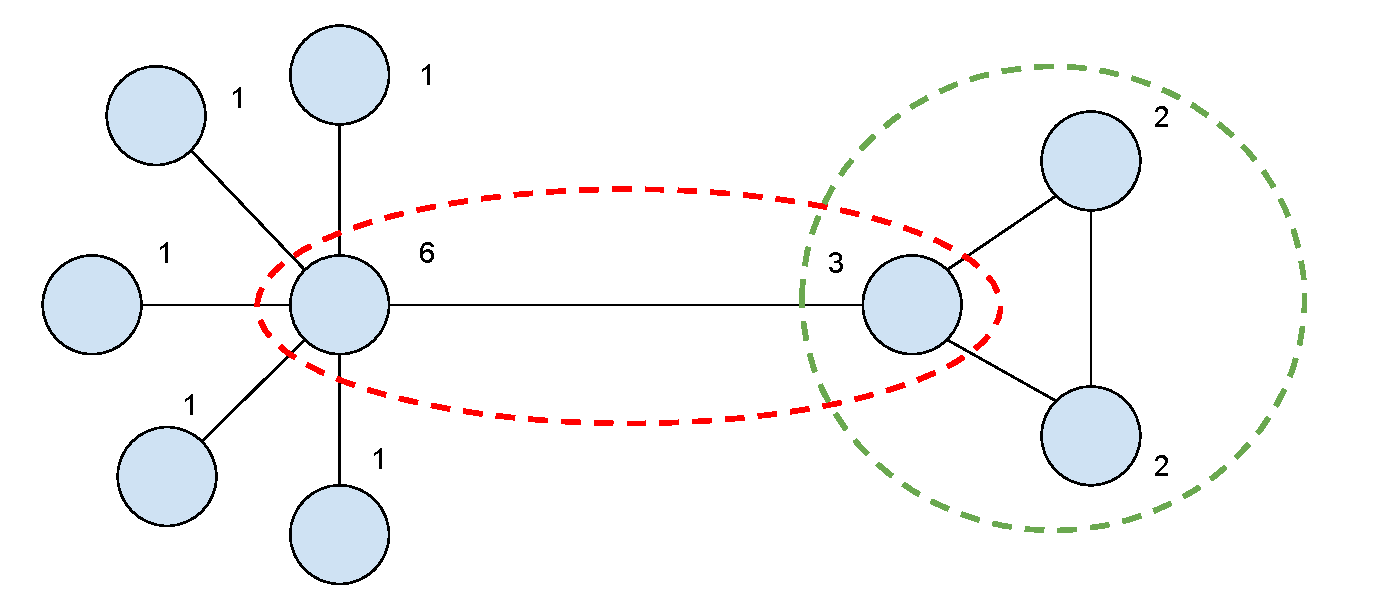
\includegraphics{graphs/greedy_grado.pdf}
\end{figure}

Sostituendolo con un ordinamento basato sul numero di triangoli incidenti non risolviamo prò il problema. Esempio:

\begin{figure}[H]
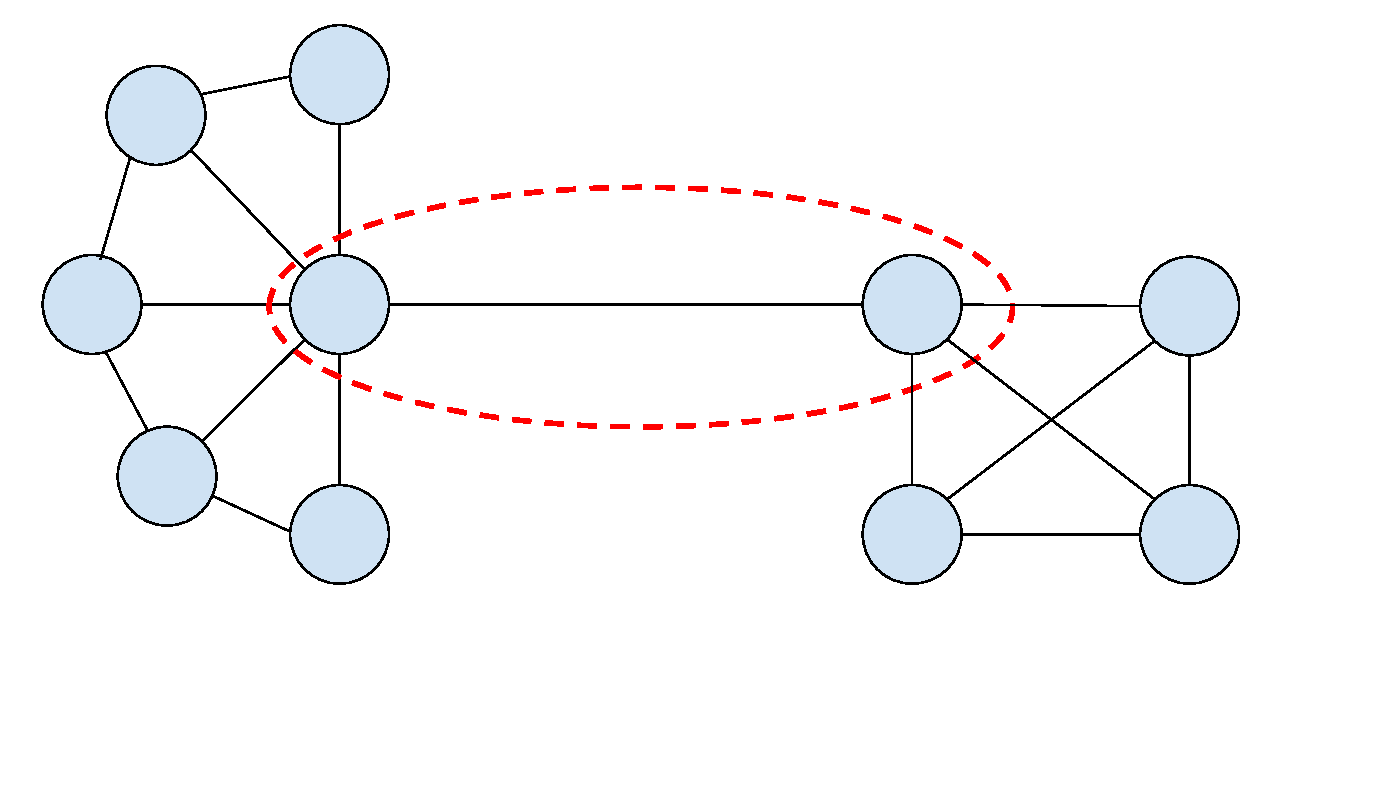
\includegraphics{graphs/greedy_triangoli.pdf}
\end{figure}

Notiamo che l'algoritmo è molto simile a Krusall. Non a caso infatti, tutti gli algoritmi Greedy han la stessa struttura:

\begin{enumerate}
\item Ordinamento
\item $ A \leftarrow \emptyset$
\item foreach $x$ (preso secondo ordinamento)
\item \hspace{\parindent} if $A \cup x$ è ok then
\item \hspace{\parindent} \hspace{\parindent} Aggiungi $x$ ad $A$
\end{enumerate}

\paragraph{Selezione attività}

Consideriamo un insieme di attività $t_1, t_2, \ldots , t_n$ con $t_i = (s_i, f_i)$ coppia in cui sono specificati i tempi di inizio e fine dell'attività. Esse sono rappresentabili attraverso un diagramma di Gantt.

\begin{ganttchart}[
x unit=0.22cm,
y unit title=0.5cm,
y unit chart=0.5cm,
title label font=\fontsize{4}{5}\selectfont,
bar label font=\tiny,
]{1}{48}
\ganttbar{Task 1}{1}{2} \\
\ganttbar{Task 2}{3}{7} \\
\ganttbar{Task 3}{8}{9} \\
\ganttbar{Task 4}{12}{15} \\
\ganttbar{Task 5}{3}{17} \\
\ganttbar{Task 6}{1}{12}
\end{ganttchart}

Vorremmo determinare un insieme di attività eseguibili in uno stesso momento, per farlo potremmo procedere all'ordinamento per:

\begin{enumerate}
\item Tempo di inizio
\item Tempo di fine
\item Durata
\end{enumerate}

Quale funzionerà meglio?
